\section{Comparison of Masking and Non-Masking Modes}
\label{secX:rendimiento-relativo}


In this section we compare the compression performance of the masking and non-masking modes of each of the evaluated coding algorithms that admit both modes. Specifically, we compare:


\vspace{-5pt}
\begin{itemize}
    \item \textit{CoderPCA-M} and \textit{CoderPCA-NM}
    \item \textit{CoderAPCA-M} and \textit{CoderAPCA-NM}
    \item \textit{CoderCA-M} and \textit{CoderCA-NM}
    \item \textit{CoderPWLH-M} and \textit{CoderPWLH-NM}
    \item \textit{CoderPWLHInt-M} and \textit{CoderPWLHInt-NM} 
    \item \textit{CoderGampsLimit-M} and \textit{CoderGampsLimit-NM}.
\end{itemize}


\vspace{+5pt}
\begin{defcion}
Let $A$ be the set of coding algorithms listed above. We define $a_\maskalgo$ and $a_\NOmaskalgo$ as the masking and non-masking modes for any given coding algorithm $a \in A$.
\end{defcion}


For comparing the performance of $a_\maskalgo$ and $a_\NOmaskalgo$ when compressing certain data with a given threshold parameter $e$, we calculate the relative difference. We only consider the window size parameters $w_\maskalgo$ and $w_\NOmaskalgo$ that obtain the best results (i.e. minimize the compression ratios). We refer to $w_\maskalgo$ and $w_\NOmaskalgo$ as the optimal window sizes and formally define them next.


\clearpage


\newcommand{\footows}{This was never the case on our experiments.}
\begin{defcion}
The \textit{optimal window size (OWS)} of a coding algorithm $a \in A$ and a threshold parameter $e \in E$, for the data of type $z$ of a certain file $f$ is given by
\begin{equation}
OWS(a, e, f_z) = w^{*} \in W \text{ such that } CR((a, w^{*}, e), f_z) = \min_{w \in W} \biggl\{ CR((a, w, e), f_z) \biggr\},
\end{equation}
where we take the smallest window in the event more than one value satisfies the equation\footnote{\footows}. Note that the triplet $(a, w, e)$ defines a CAI in $\ca$, hence we are correctly applying equation~(\ref{eq:compression-rate}).
\end{defcion}


For each data type $z$ of each dataset file $f$, and each threshold parameter $e \in E$ and coding algorithm $a \in A$, we calculate the equation~(\ref{eq:relative-difference}) as
\begin{equation}
\label{eq:relative-difference-apply}
\difrelativa((a_\maskalgo, w_\maskalgo^{*}, e), (a_\NOmaskalgo, w_\NOmaskalgo^{*}, e), f_z),
\end{equation}
where $w_\maskalgo^{*}=OWS(a_\maskalgo, e, f_z)$ and $w_\NOmaskalgo^{*}=OWS(a_\NOmaskalgo, e, f_z)$. Note that both triplets $(a_\maskalgo, w_\maskalgo^{*}, e)$ and $(a_\NOmaskalgo, w_\NOmaskalgo^{*}, e)$ define CAIs in $\ca$, hence we are correctly applying the relative difference equation.


As an example, in Figure~\ref{fig:diff-sst} and Figure~\ref{fig:diff-tornado} we display the compression ratio and relative difference plots obtained for two data types of different datasets. We selected these two plots because they include the maximum and minimum values returned by equation~(\ref{eq:relative-difference-apply}).


Table~\ref{tabla:rendimiento-relativ-NM-M} summarizes the results obtained for each dataset when comparing the relative performance of $a_\maskalgo$ and $a_\NOmaskalgo$ for each $a \in A$. The second column outlines the amount of gaps in the dataset. The third column displays the percentage of combinations in which $a_\maskalgo$ performs better than $a_\NOmaskalgo$ (i.e. cases in which equation~(\ref{eq:relative-difference-apply}) returns a positive value). The last column shows the range for the values of equation (\ref{eq:relative-difference-apply}) for said combinations.


\vspace{+5pt}

\begin{table}[h]
\begin{center}
    \begin{tabular}{| C{2.2cm} || C{2.5cm} | C{4.4cm} | C{3.0cm} |}
    \hline
      \multicolumn{1}{|>{\centering\arraybackslash}m{2.2cm}||}{\textbf{Dataset}} 
    & \multicolumn{1}{>{\centering\arraybackslash}m{2.5cm}|}{\textbf{Dataset Characterstic}} 
    & \multicolumn{1}{>{\centering\arraybackslash}m{4.4cm}|}{\textbf{Cases where masking outperforms non-masking variant (\%)}}
    & \multicolumn{1}{>{\centering\arraybackslash}m{3.0cm}|}{\textbf{RD (\%) Range}}\\
    \hline
    \datasetirkis   & Many gaps     & 100 & (0; 36.88]                    \\\hline
    \datasetsst     & Many gaps     & 100 & (0; \textcolor{red}{50.60}]  \\\hline
    \datasetadcp    & Many gaps     & 100 & (0; 17.35]                    \\\hline
    \datasetelnino  & Many gaps     & 100 & (0; 50.52]                    \\\hline
    \datasetsolar   & Few gaps      & 51  & [-0.25; 1.77]                 \\\hline
    \datasethail    & No gaps       & 0   & [-0.04; 0)                    \\\hline
    \datasettornado & No gaps       & 0   & [\textcolor{blue}{-0.29}; 0)   \\\hline
    \datasetwind    & No gaps       & 0   & [-0.12; 0)                    \\\hline
    \toprule[0.1mm]
    \end{tabular}
    \caption{Relative difference between the masking and non-masking variants of each algorithm. In the last column we highlight the maximum (red) and minimum (blue) values taken by RD.}
    \label{tabla:rendimiento-relativ-NM-M}
\end{center}
\end{table}

\vspace{-5pt}


For every coding algorithm, on datasets with many gaps the masking mode always produces the best result, while on gapless datasets the non-masking mode always achieves the best result. On the dataset with few gaps, on each half of the combinations the best results are obtained with different modes.


Observing the last column of Table~\ref{tabla:rendimiento-relativ-NM-M}, we notice that in every case in which the non-masking mode $a_\NOmaskalgo$ performs best, the relative difference is close to zero. In Figure~\ref{fig:diff-tornado} we show the case in which $a_\NOmaskalgo$ obtains the most significative relative difference. This occurs for the \datasettornado \ dataset and in the table we can verify that in such case the relative difference is -0.29\%.


\clearpage




\newcommand{\commonfigurescomp}{Compression rate and relative difference for the combinations <$\coder \in C$, $u \in U$>\\for the }

\begin{figure}
\hspace{-70pt}
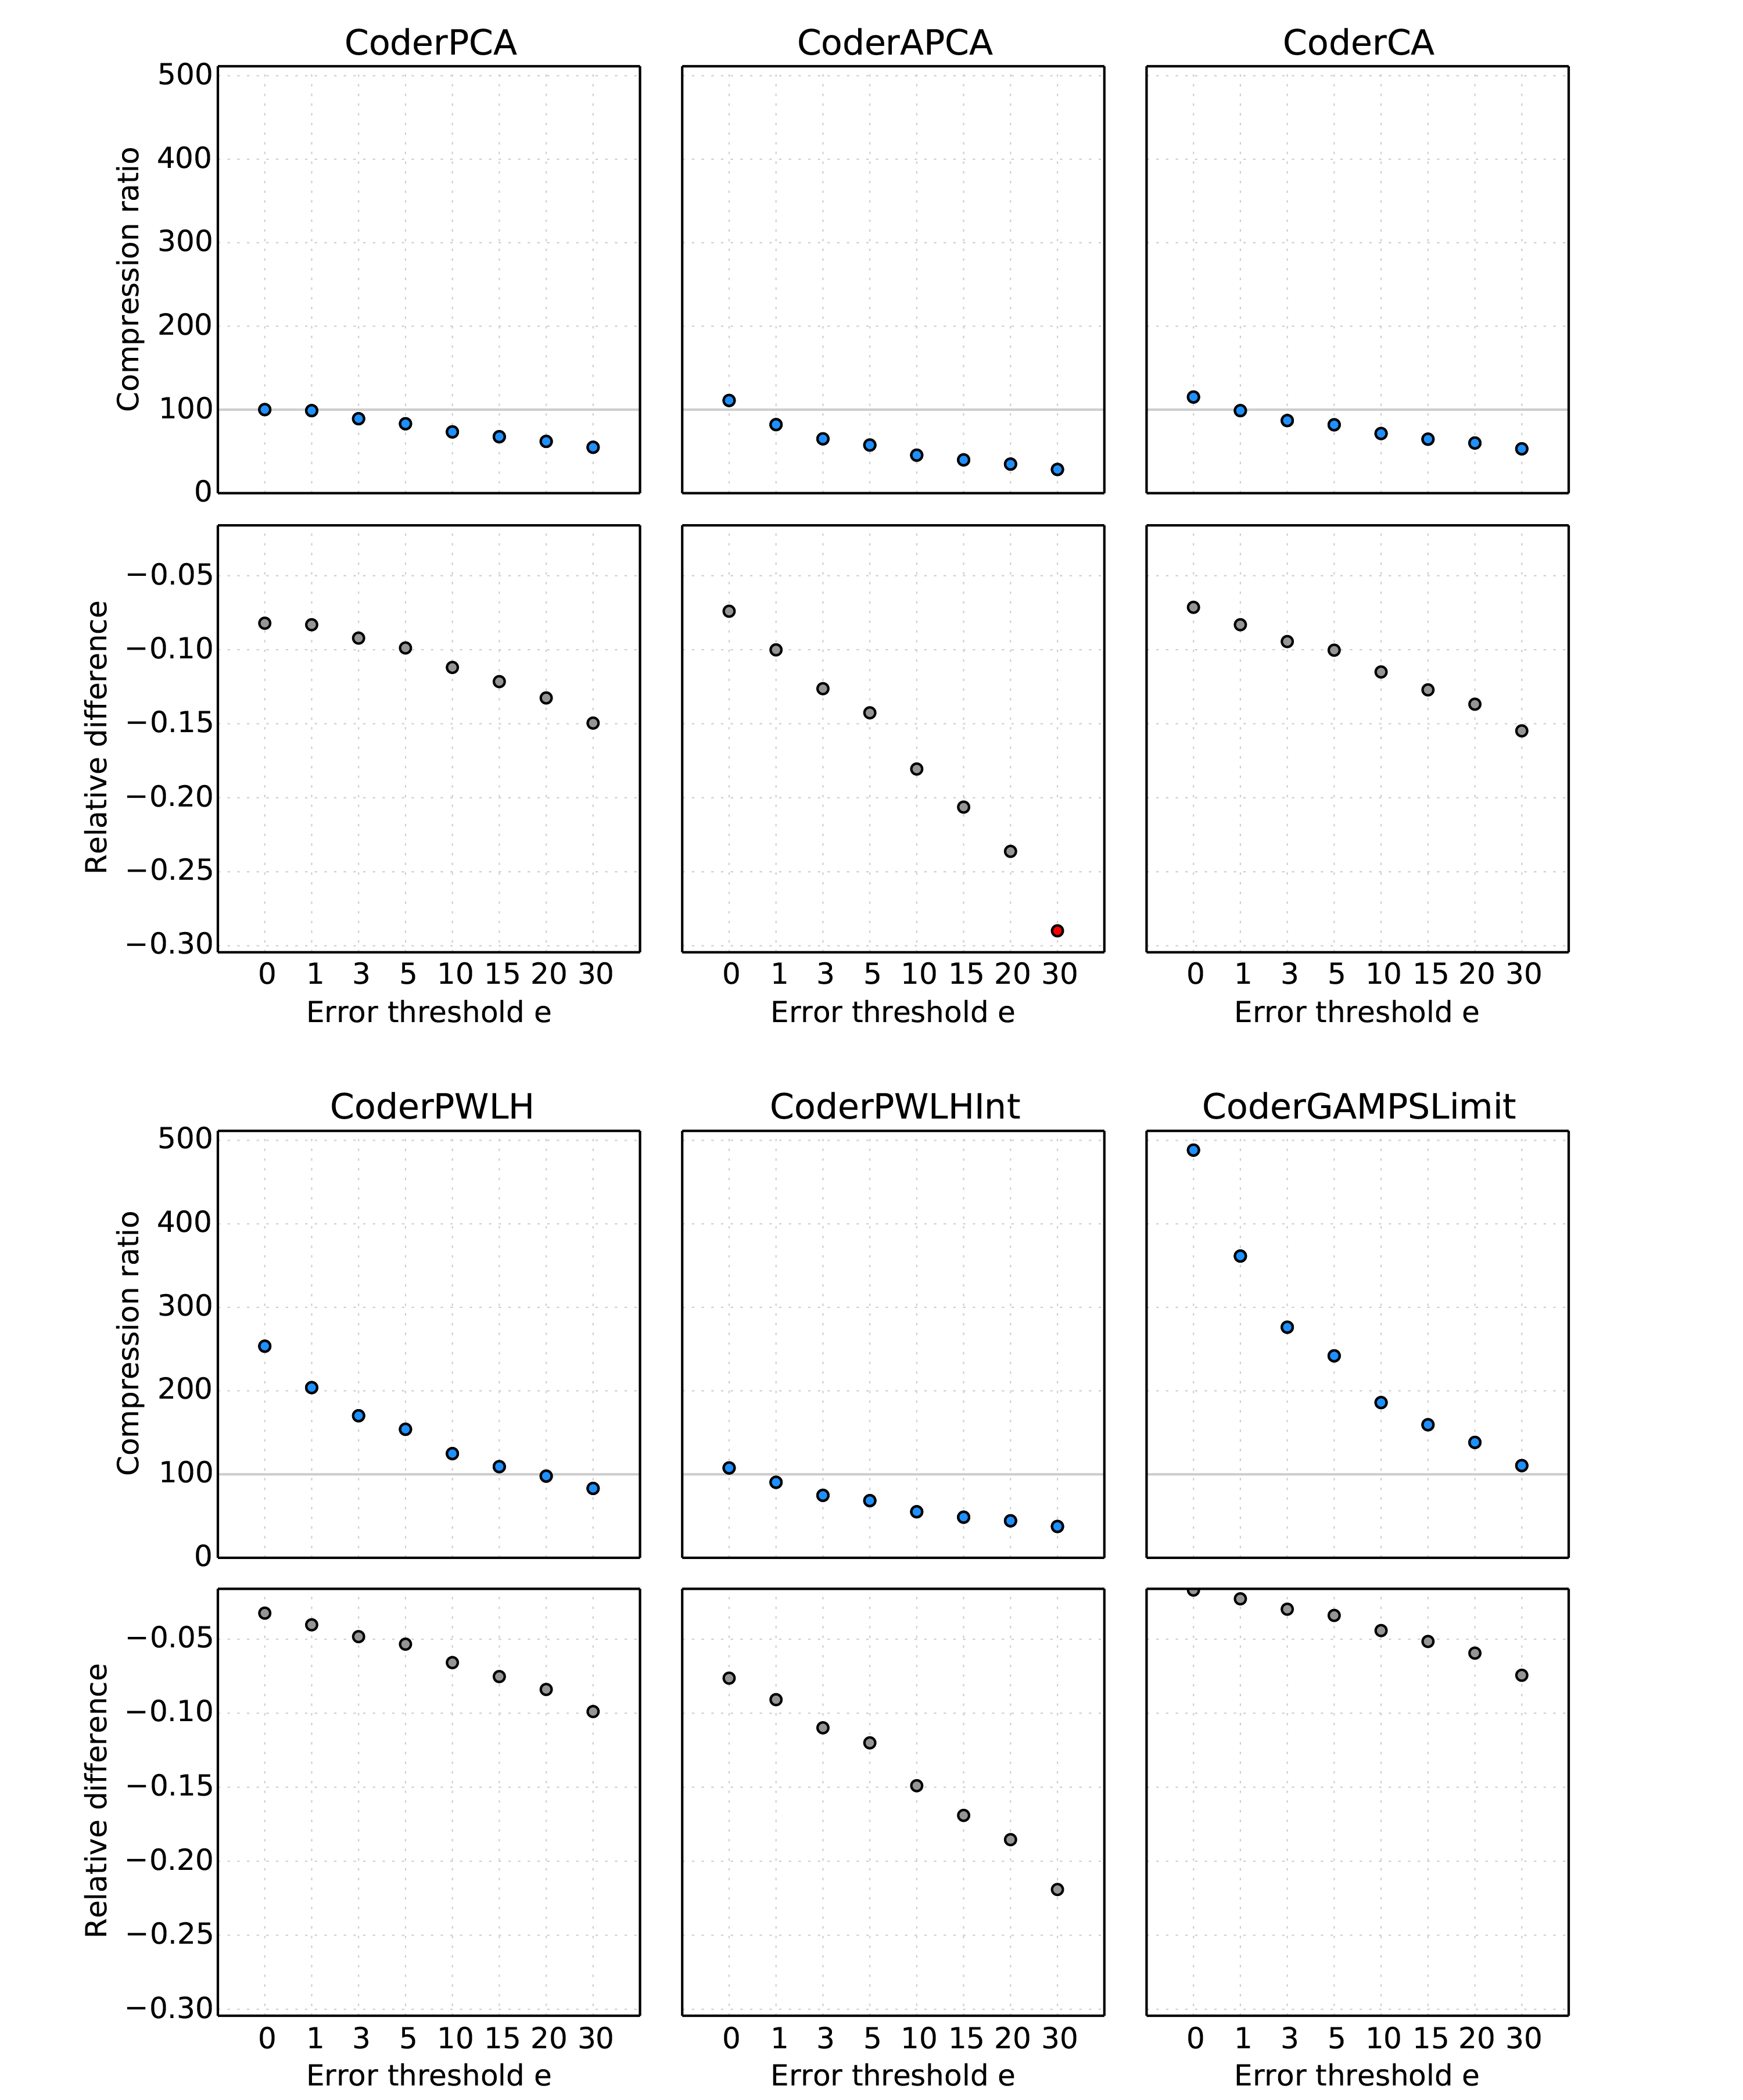
\includegraphics[scale=0.75]{chapters/Experiments/images/32-Tornado.png}
\hspace{+10pt}
\caption{\commonfigurescomp ``Longitude" data type of the \datasettornado \ dataset. In the relative difference plot for\\CoderAPCA we marked with red color the case in which \cNOmaskalgo \ obtains \\the most significant relative difference (-0.29).}
\label{fig:diff-tornado}
\end{figure}

\clearpage

\begin{figure}
\hspace{-70pt}
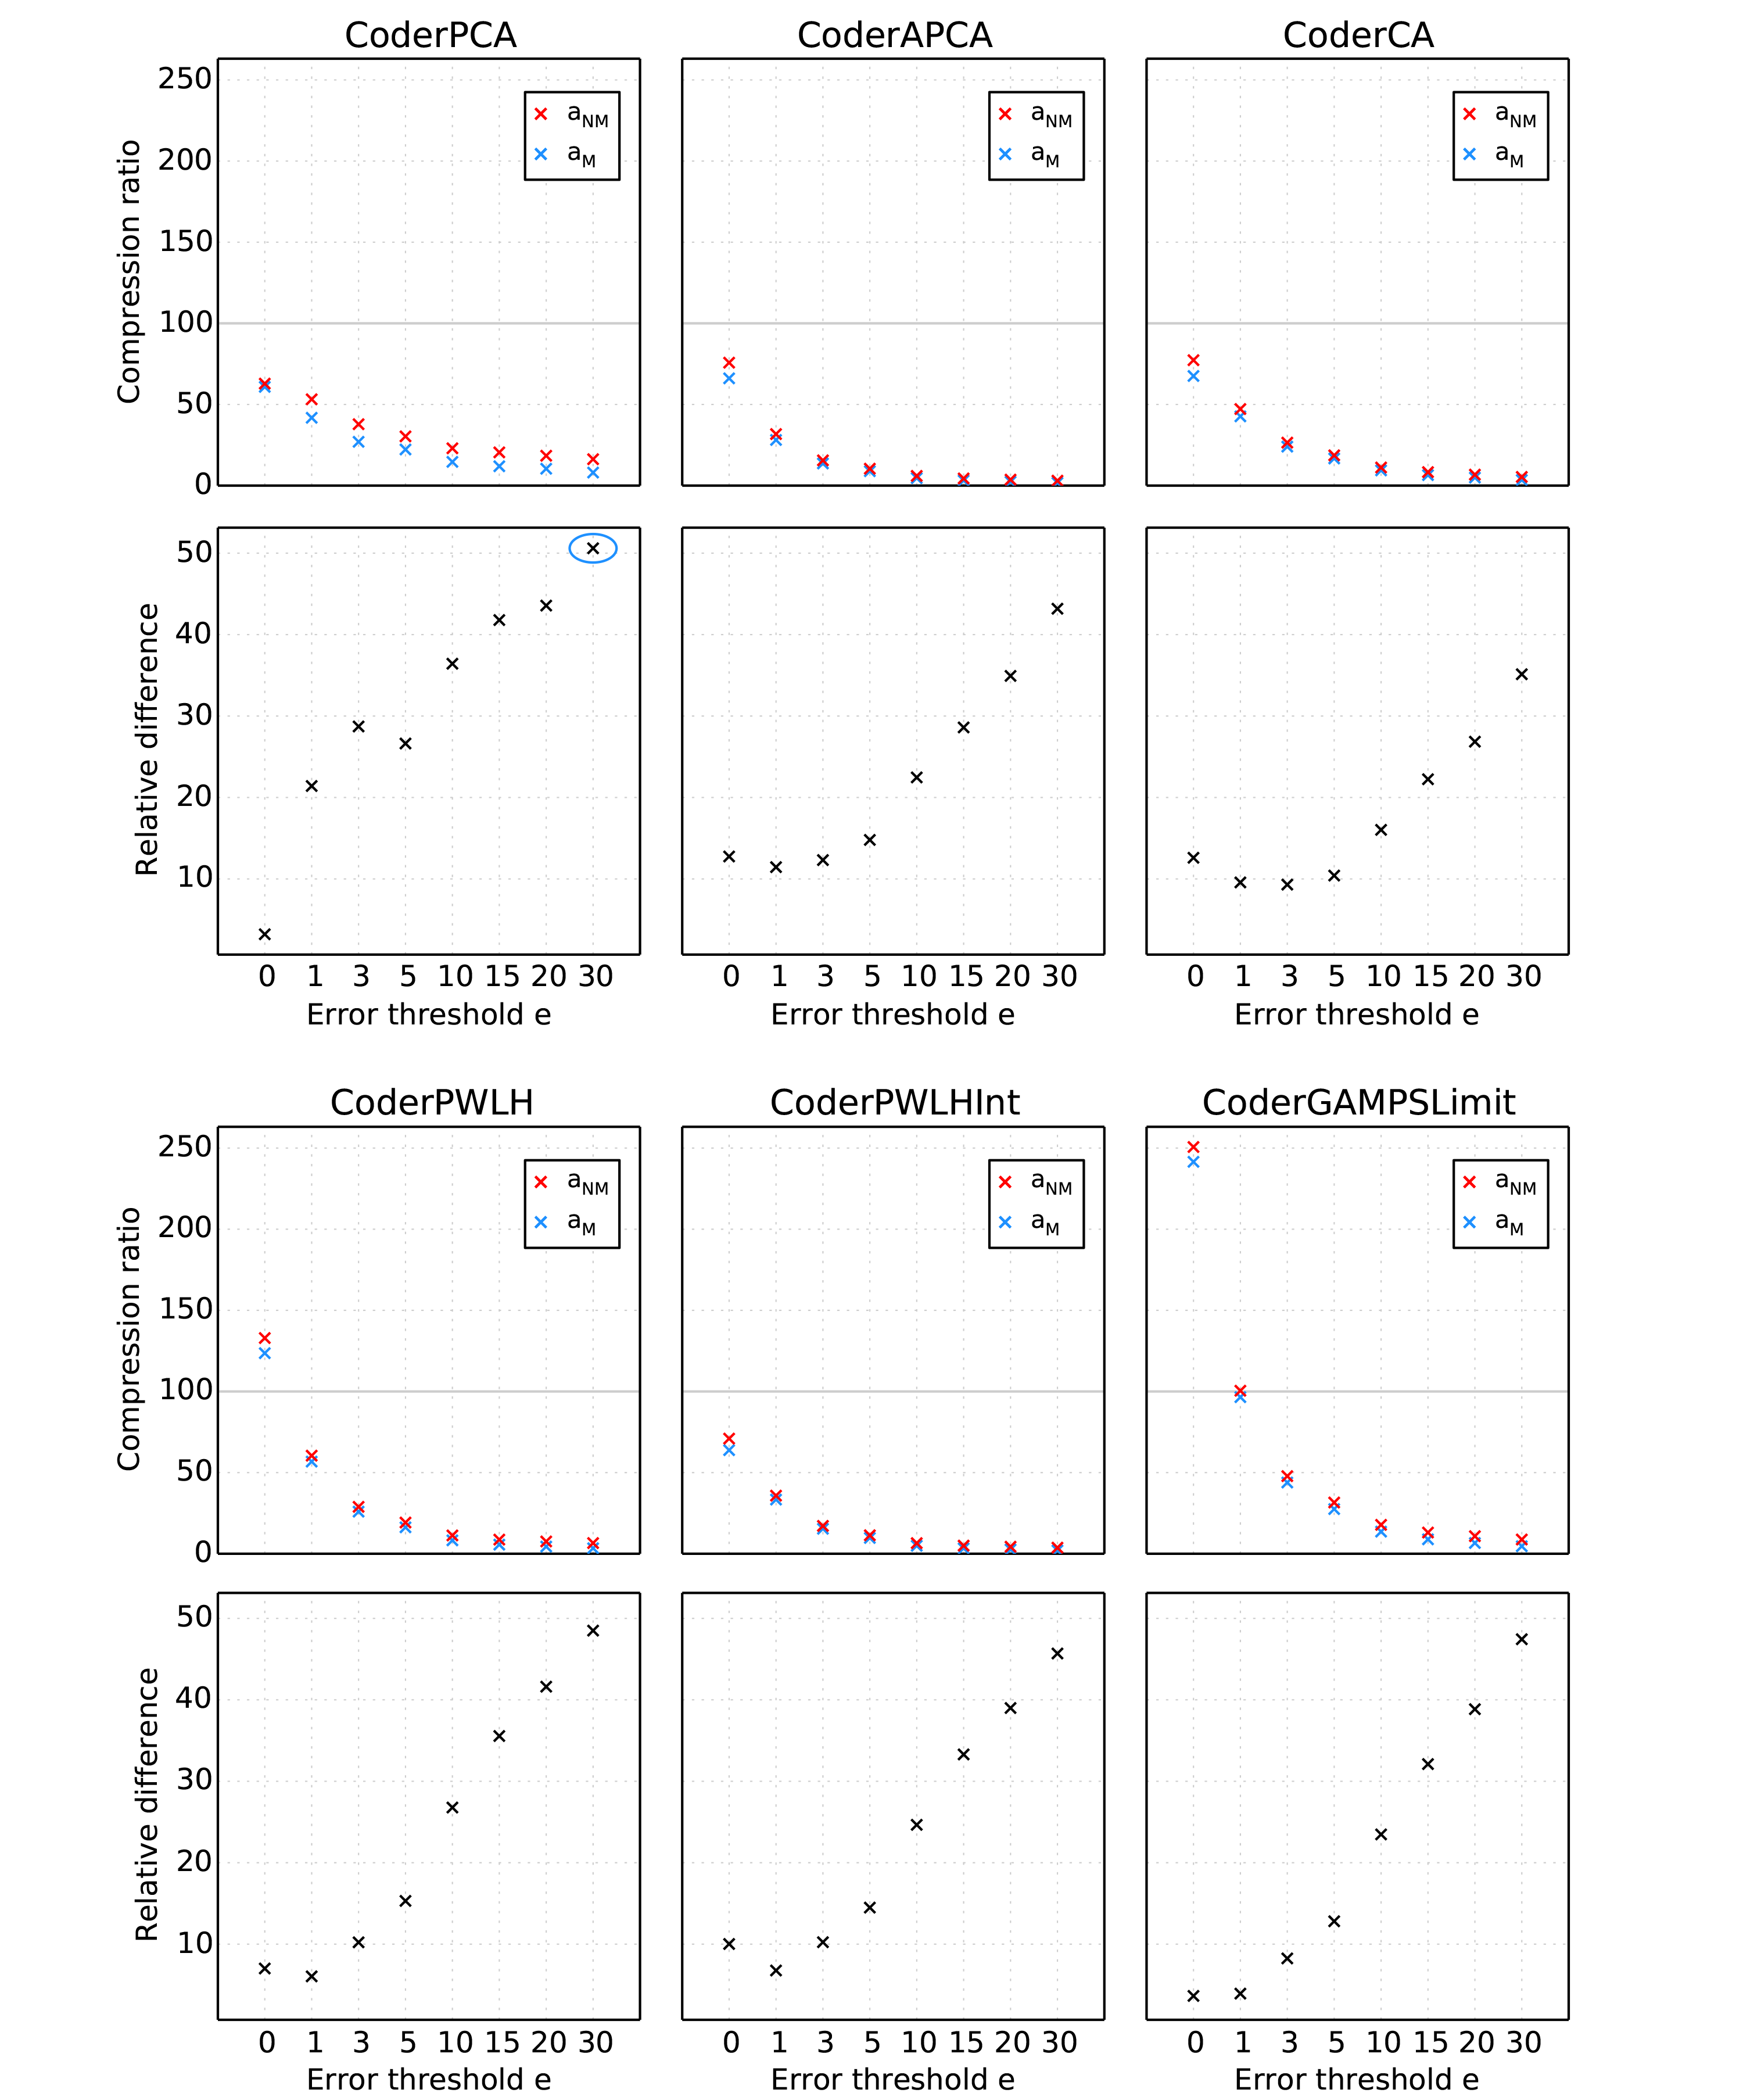
\includegraphics[scale=0.75]{chapters/Experiments/images/32-SST.png}
\hspace{+10pt}
\caption{\commonfigurescomp ``VWC" data type of the \datasetsst \ dataset. In the relative difference plot for\\CoderPCA we marked with blue color the case in which \cmaskalgo \ obtains \\the most significant relative difference (50.60).}
\label{fig:diff-sst}
\end{figure}



\clearpage


On the other hand, when the masking mode $a_\maskalgo$ performs best, the relative difference reaches high absolute values. The maximum, which amounts to 50.60\%, is achieved for the \datasetsst \ dataset. We show that particular case in Figure~\ref{fig:diff-sst}.


The experimental results presented in this section suggest that if we were interested in compressing a dataset with many gaps, we would benefit by using a masking coding algorithm $a_\maskalgo$. However, even if the dataset didn't have any gaps, the performance gain obtained by using a non-masking algorithm $a_\NOmaskalgo$ instead would be negligible. Since the $a_\maskalgo$ algorithm is more robust and performs better in general, in the next sections we will focus on its study.
